\documentclass[a4paper,12pt]{article}

\usepackage{datenumber} % requires texlive-latex-extra
\usepackage{fancyhdr}
\usepackage{footnote}
\usepackage{fp}
\usepackage{graphicx}
\usepackage[hidelinks]{hyperref}
\usepackage{multicol}
\usepackage[utf8]{inputenc}
\usepackage{url}

% personal data
\newcommand\myFullName{Igor Botian}
\newcommand\myBirthYear{1987}
\newcommand\myBirthMonth{12}
\newcommand\myBirthMonthAsString{Dec}
\newcommand\myBirthDay{09}

% PDF properties
\hypersetup{
    pdfauthor={\myFullName},
    pdftitle={CV}
}

% paragraphs
\setlength\parindent{0pt}

% headers and footers
\pagestyle{fancy}
\fancyhf{}
\rhead{\myFullName, igor.botian@gmail.com}
\cfoot{\thepage}
\renewcommand{\headrulewidth}{0pt}
\setlength{\headheight}{15pt}

% footnotes
\makesavenoteenv{tabular}

% age
\newcounter{myBirthDate}
\newcounter{todayDate}
\setmydatenumber{myBirthDate}{1987}{12}{09}
\setmydatenumber{todayDate}{\the\year}{\the\month}{\the\day}
\FPsub\result{\thetodayDate}{\themyBirthDate}
\FPdiv\myage{\result}{365.2425}

%%%%%%%%%%%%%%%%%%%%%%%%%%%%%%%%%%%%%%%%%%%%%%%%%%%%%%%%%%%%%%%%%%%%%%%%%%%%%%%

\begin{document}

\section*{CV}

\begin{multicols}{2}
    \begin{tabular}{ll}
        \textbf{Position} & Java developer \\
        \textbf{Full name} & \myFullName \\
        \textbf{Age} & \FPtrunc\myage{\myage}{0}\myage\ years old \\
        \textbf{Date of birth} & \myBirthMonthAsString\ \myBirthDay\ \myBirthYear \\
        \textbf{Status} & married \\
        \textbf{Citizenship} & Russian Federation \\
        \textbf{Location} & Saint Petersburg, Russia \\
        \textbf{Phone number} & +7 (967) 511-19-64 \\
        \textbf{E-mail} & igor.botian@gmail.com \\
    \end{tabular}
    \null\hfill 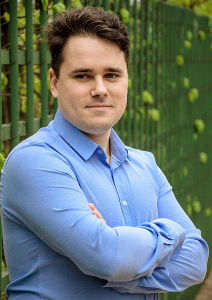
\includegraphics[width=0.5\linewidth]{photo.jpg}
\end{multicols}

%%%%%%%%%%%%%%%%%%%%%%%%%%%%%%%%%%%%%%%%%%%%%%%%%%%%%%%%%%%%%%%%%%%%%%%%%%%%%%%

\section*{Work experience}

\subsection*{Jun 2012 - Present, Alcatel-Lucent Enterprise}

\begin{tabular}{ll}
    \textbf{Position} & Java developer; Tech. lead; Scrum master (certified\footnote{\url{http://bcert.me/szowjwtj}}) \\
    \textbf{Project} & OpenTouch Solutions\footnote{\url{https://www.al-enterprise.com/en/products/platforms/opentouch-multimedia-services}} \\
    \textbf{Technologies} & Java SE, OpenJPA, PostgreSQL, RabbitMQ, Tomcat, \\
        & OpenSUSE Linux, Mercurial, Maven \\
\end{tabular}

\subsection*{Sep 2009 - Jan 2012, Radar MMS}

\begin{tabular}{ll}
    \textbf{Position} & Java developer \\
    \textbf{Project} & Ballistic intercontinental rocket engineering\footnote{\url{http://www.radar-mms.com/Product.aspx?product_7}} \\
        & (target detection module based on antenna-phased arrays) \\
        & (software modeling) \\
    \textbf{Customer} & The Ministry of Defense of the Russian Federation \\
    \textbf{Technologies} & Java SE, Swing, Ant, Git \\
\end{tabular}

\subsection*{Mar 2008 - Aug 2010, NIC SPb ETU}

\begin{tabular}{ll}
    \textbf{Year} & 2010 \\
    \textbf{Position} & Java/C++ developer \\
    \textbf{Project} & Satellite data processing and storage system\footnote{\url{http://www.nicetu.spb.ru/index.php/ru/resheniya-i-proekty/cistemy-sbora-i-obrabotki-izmeritelnoj-informatsii}} \\
    \textbf{Customer} & The Ministry of Defense of the Russian Federation \\
    \textbf{Technologies} & Java SE, GWT, PostgreSQL, JNI, Ant, SVN, \\
        & OS MSVS (Russian military OS based on Fedora Linux) \\
\end{tabular}

\bigskip

\begin{tabular}{ll}
    \textbf{Year} & 2009 \\
    \textbf{Position} & Java developer \\
    \textbf{Project} & Satellite trajectory construction system\footnote{\url{http://www.nicetu.spb.ru/index.php/ru/resheniya-i-proekty/kompleksy-rascheta-etalonnykh-traektorij-dlya-vypolneniya-yustirovochnykh-rabot}} \\
    \textbf{Customer} & The Russian Federal Space Agency \\
    \textbf{Technologies} & Java SE, Swing, Maven, SVN \\
\end{tabular}

\bigskip

\begin{tabular}{ll}
    \textbf{Year} & 2008 \\
    \textbf{Position} & Java developer \\
    \textbf{Project} & Electronic declaration system\footnote{\url{http://www.nicetu.spb.ru/index.php/ru/resheniya-i-proekty/sistema-monitoringa-i-kontrolya-soversheniya-tamozhennykh-operatsij}} \\
    \textbf{Customer} & The Federal Customs Service of Russia \\
    \textbf{Technologies} & JSP, Tomcat, Oracle, JavaScript, Ant, SVN \\
\end{tabular}

%%%%%%%%%%%%%%%%%%%%%%%%%%%%%%%%%%%%%%%%%%%%%%%%%%%%%%%%%%%%%%%%%%%%%%%%%%%%%%%

\section*{Educational background}

\subsection*{2012 - 2015}

\begin{tabular}{ll}
    \textbf{University} & Saint Petersburg State Forestry Technical University, Russia \\
    \textbf{Degree} & Ph. D. (Technology) \\
    \textbf{Major Subject} & Industrial process management and automation \\
\end{tabular}

\subsection*{2010 - 2012}

\begin{tabular}{ll}
    \textbf{University} & Lappeenranta University of Technology, Finland \\
    \textbf{Degree} & M. Sc. (Technology) \\
    \textbf{Major Subject} & Communication software
\end{tabular}

\subsection*{2009 - 2011}

\begin{tabular}{ll}
    \textbf{University} & Saint Petersburg State Electrotechnical University, Russia \\
    \textbf{Degree} & M. Sc. (Technology) \\
    \textbf{Major Subject} & Applied mathematics and informatics \\
\end{tabular}

\subsection*{2005 - 2009}

\begin{tabular}{ll}
    \textbf{University} & Saint Petersburg State Electrotechnical University, Russia \\
    \textbf{Degree} & B. Sc. (Technology) \\
    \textbf{Major Subject} & Engineering and technology \\
\end{tabular}

%%%%%%%%%%%%%%%%%%%%%%%%%%%%%%%%%%%%%%%%%%%%%%%%%%%%%%%%%%%%%%%%%%%%%%%%%%%%%%%

\section*{Language skills}

\begin{tabular}{ll}
    \textbf{Russian} & Native \\
    \textbf{English} & Upper-intermediate, fluent \\
    \textbf{Finnish} & Basic \\
\end{tabular}

%%%%%%%%%%%%%%%%%%%%%%%%%%%%%%%%%%%%%%%%%%%%%%%%%%%%%%%%%%%%%%%%%%%%%%%%%%%%%%%

\section*{Publications}

\begin{tabular}{ll}
    \textbf{In English} & I. Botian, `Software security vulnerabilities in mobile \\
        & peer-to-peer environment``, ISBN 978-3-659-11253-9 \\
    \textbf{In Russian} & 6 publications (machine learning, SVM) \\
\end{tabular}

\end{document}
